% Author: Izaak Neutelings (October 2021)
% Inspiration
%   "Very special relativity - An illustrated guide", Sander Bais (2007)
%   http://people.uncw.edu/hermanr/GR/Minkowski/Minkowski.pdf
\documentclass[border=3pt,tikz]{standalone}
\usepackage{amsmath} % for \text
\usepackage{etoolbox} % ifthen
\usepackage[outline]{contour} % glow around text
\usetikzlibrary{calc} % for adding up coordinates
\usetikzlibrary{decorations.markings,decorations.pathmorphing}
\usetikzlibrary{angles,quotes} % for pic (angle labels)
\usetikzlibrary{arrows.meta} % for arrow size
\usepackage{xfp} % higher precision (16 digits?)
\contourlength{1.1pt}

\tikzset{>=latex} % for LaTeX arrow head
\colorlet{myred}{red!85!black}
\colorlet{mydarkred}{red!55!black}
\colorlet{mylightred}{red!85!black!12}
\colorlet{myfieldred}{mydarkred!5} % for S' background
\colorlet{myredhighlight}{myred!20} % highlights simultaneity in ladder paradox
\colorlet{myblue}{blue!80!black}
\colorlet{mydarkblue}{blue!50!black}
\colorlet{mylightblue}{blue!50!black!30}
\colorlet{mylightblue2}{myblue!10}
\colorlet{mygreen}{green!80!black}
\colorlet{mypurple}{blue!40!red!80!black}
\colorlet{mydarkgreen}{green!50!black}
\colorlet{mydarkpurple}{blue!40!red!50!black}
\colorlet{myorange}{orange!40!yellow!95!black}
\colorlet{mydarkorange}{orange!40!yellow!85!black}
\colorlet{mybrown}{brown!20!orange!90!black}
\colorlet{mydarkbrown}{brown!20!orange!55!black}
\colorlet{mypurplehighlight}{mydarkpurple!20} % highlights simultaneity in ladder paradox
\tikzstyle{world line}=[myblue!40,line width=0.3]
\tikzstyle{world line t}=[mypurple!50!myblue!40,line width=0.3]
\tikzstyle{world line'}=[mydarkred!40,line width=0.3]
\tikzstyle{mysmallarr}=[-{Latex[length=3,width=2]},thin]
\tikzstyle{mydashed}=[dash pattern=on 3 off 3]
\tikzstyle{rod}=[mydarkbrown,draw=mydarkbrown,double=mybrown,double distance=2pt,
                 line width=0.2,line cap=round,shorten >=1pt,shorten <=1pt]
%\tikzstyle{rod'}=[rod,draw=mydarkbrown!80!red!85,double=mybrown!80!red!85]
\tikzstyle{vector}=[->,line width=1,line cap=round]
\tikzstyle{vector'}=[vector,shorten >=1.2]
\tikzstyle{particle}=[mygreen,line width=0.9]
\tikzstyle{photon}=[-{Latex[length=5,width=4]},myorange,line width=0.8,decorate,
                    decoration={snake,amplitude=1.0,segment length=5,post length=5}]

\def\tick#1#2{\draw[thick] (#1) ++ (#2:0.06) --++ (#2-180:0.12)}
\def\tickp#1#2{\draw[thick,mydarkred] (#1) ++ (#2:0.06) --++ (#2-180:0.12)}
\def\Nsamples{100} % number samples in plot

\begin{document}

% SPACETIME DIAGRAM - EUCLIDEAN ROTATION
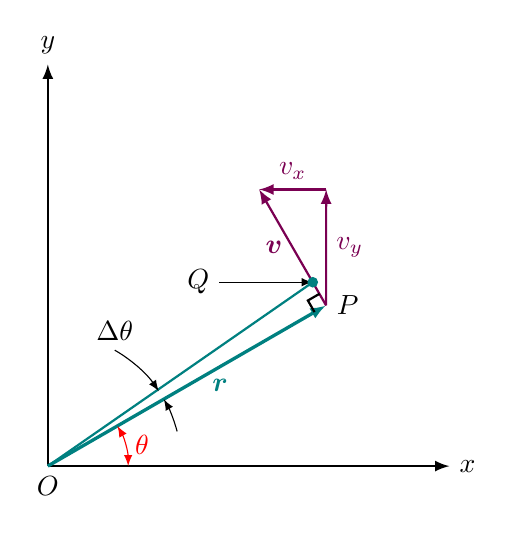
\begin{tikzpicture}[scale=1.7]
  

    
    \pgfmathsetmacro\ang{30} % angle between x and x' axes
    \pgfmathsetmacro\r{2.4}
    \pgfmathsetmacro\vv{1.0}
    \coordinate (O) at (0,0);
    \coordinate (X) at (2,0);
    \coordinate (P) at (\ang:\r);
    \coordinate (V0) at ($(P) + ({90+\ang}:\vv)$);
    \coordinate (V1) at ($(P) + (0, \vv*cos{\ang})$);
    \coordinate (Q) at ($(P) + ({90+\ang}:0.2)$);
    \coordinate (R1) at ($(P)+({180+\ang}:0.1)$);
    \coordinate (R2) at ($(R1) + ({90+\ang}:0.1)$);
    \coordinate (R3) at ($(R2) + (\ang:0.1)$);
    
    % AXES
    \draw[->,thick] (O) node [below] {$O$} -- (0,3) node[above] {$y$};
    \draw[->,thick] (O) -- (3, 0) node[right] {$x$};
    % \draw[->,thick,mydarkred] (90+\ang:0) -- (T')
    %     node[above] {$y'$};
    % \draw[->,thick,mydarkred] (\ang:0) -- (X')
    %     node[above=3,right=0] {$x'$};

        % EVENT
    
    \draw[->, thick, mypurple] (P) -- node [left] {$\boldsymbol{v}$} (V0);
    \draw[->, thick, mypurple] (P) -- node [right] {$v_y$} (V1);
    \draw[->, thick, mypurple] (V1) -- node [above] {$v_x$} (V0);


    \draw[-{Latex[width=1.5mm, length=2mm]}, very thick, teal] (O) -- node [xshift=12] {$\boldsymbol{r}$} (P) node [right, black] {$P$}; 
    
    \draw[black, thick] (R1) -- (R2) -- (R3);
    \draw [<-] (Q) -- ($(Q)+ (-0.7, 0)$) node [left] {$Q$};
    
    \draw[thick, teal] (O) -- (Q);
    \filldraw[fill=teal, color=teal]  (Q) circle (1pt);
    
    \draw[<->, red] (0.6, 0) arc (0:\ang:0.6) node [midway, right] {$\theta$};
    \draw[->] ({\ang+30}:1) node[above] {$\Delta \theta$} arc ({\ang+30}:{\ang+4}:1) ;
    \draw[->] ({\ang-15}:1)  arc ({\ang-15}:{\ang}:1) ;


\end{tikzpicture}


\end{document}